\documentclass{beamer}

\usepackage{wrapfig}
\usepackage{algpseudocode}
\usepackage{algorithm}
\usepackage[export]{adjustbox}
\usepackage{svg}

\usetheme{Boadilla}
\usecolortheme{dolphin}
\setbeamertemplate{navigation symbols}{}
\setbeamertemplate{sections/subsections in toc}[sections numbered]

\setbeameroption{hide notes}
% \setbeameroption{show only notes}
% \setbeameroption{show notes on second screen=right}

\title[Embedded Trace]
{Embedded Trace: Assessing Data Dependence and Age}
\author[]{Hossein Afkar}
\institute{DRTS Lab}
\date{\today}

\begin{document}

\frame{\titlepage}

\begin{frame}
    \frametitle{Outline}
    \tableofcontents[hideallsubsections]
\end{frame}

\AtBeginSection[]
{
    \begin{frame}{Outline}
        \tableofcontents[currentsection]
    \end{frame}
}

\section{Preface}
\begin{frame}
    \frametitle{Preface}
    \begin{itemize}
        \item Data Age and Cause-Effect Chains.
        \item Understanding How ETM works.
    \end{itemize}
\end{frame}

\section{Data Age and Cause-Effect Chains}
\begin{frame}
    \frametitle{Synthesizing Job-Level Dependencies for Automotive
    Multi-Rate Effect Chains}
    \begin{itemize}
        \item Real-time systems require a formal guarantee of
            timing-constraints, not only for individual tasks but also
            for data-propagation.
        \item Meeting timing constraints is difficult with multi-rate tasks
            chains in which tasks are activated with different periods.
        \item 
    \end{itemize}
\end{frame}
\section{Understanding ETM}
\begin{frame}
    \frametitle{ETM Progression in Time}
    \begin{itemize}
        \item Advanced architectural improvements have found their way
            into the embedded systems. ETM also needed to evolve with these
            improvements and features.
        \item ETMv1 started with ARM7TDMI. An architecture without speculation
            and a simple three stage pipeline.
        \item ETMv4 is present in ARMv8.x which is a speculating machine with
            a more advanced pipeline.
        \item Therefore ETM needs to provide different information with
            different iteration of the hardware.
    \end{itemize}
\end{frame}
\begin{frame}
    \frametitle{ETMv1: Providing View Into the Pipeline}
    \begin{itemize}
        \item ETMv1 provides a view into the core via the execution stage of
            the pipeline.
        \item Every Instruction is cycle counted regardless.
    \end{itemize}
        \begin{figure}
        \centering
        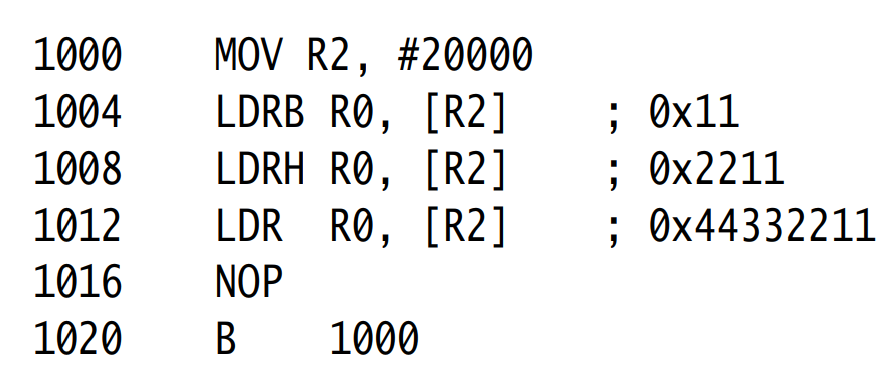
\includegraphics[width=0.80\columnwidth]{etmv11.png}
        \caption{Sample Traced Code}
        \label{fig:ETMv11}
    \end{figure}
\end{frame}
\begin{frame}
    \frametitle{ETMv1: Sample Trace} 
        \begin{figure}
        \centering
        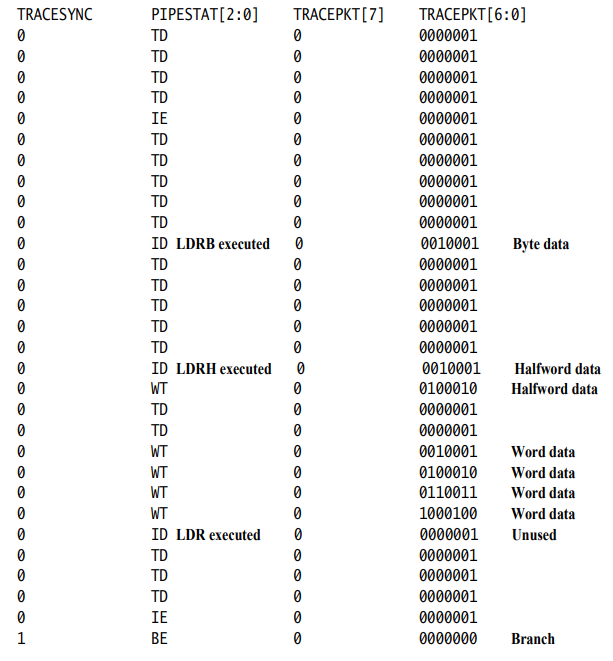
\includegraphics[width=0.55\columnwidth]{etmv12.png}
        \caption{Sample Traced Code}
        \label{fig:ETMv12}
    \end{figure}
\end{frame}
\begin{frame}
    \frametitle{ETMv4: Changing The View}
    \begin{itemize}
        \item For advanced architectures a view into the pipeline was no longer
            sufficient.
        \item To statisfy the needs of a speculating cpu core ETMv4
            specification is designed.
        \item Cycle counting is only possible when instructions batches are
            commited (This happens at branch boundaries and with enough
            configuration on Loads and Stores).
        \item So we can measure basic blocks easily in speculative processors.
    \end{itemize}
\end{frame}
\begin{frame}
    \frametitle{ETMv4: Sample Trace} 
        \begin{figure}
        \centering
        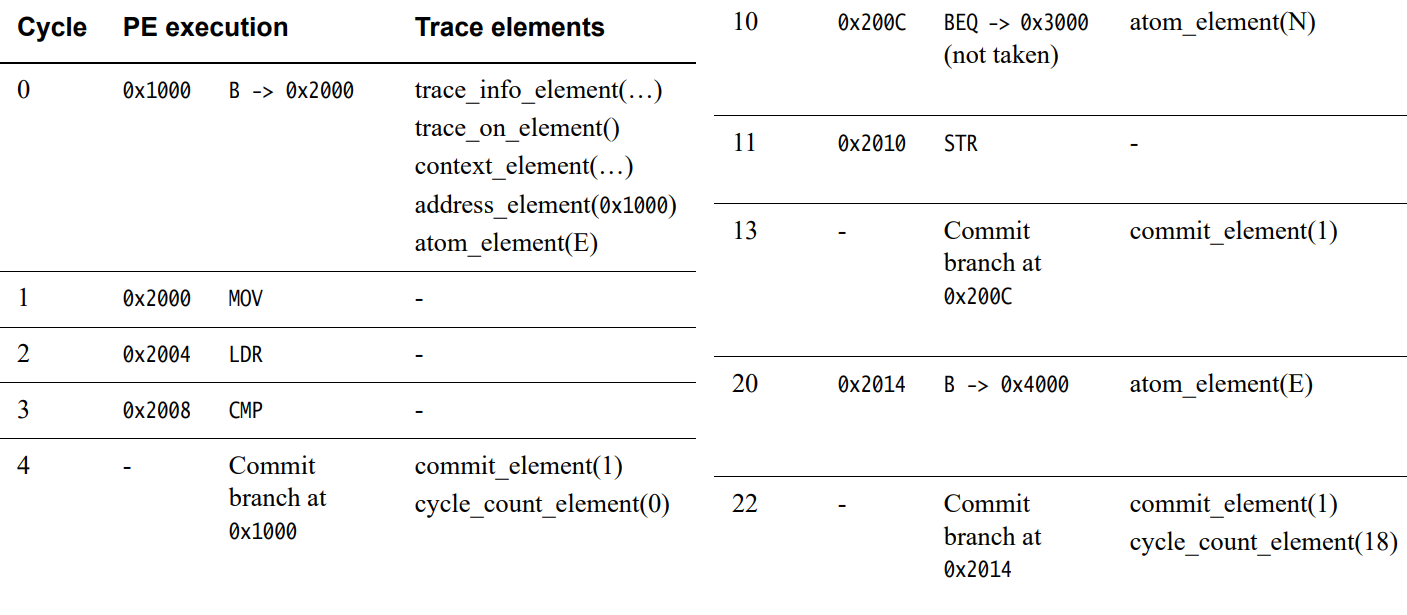
\includegraphics[width=0.90\columnwidth]{etmv4.png}
        \caption{Sample Traced Code}
        \label{fig:ETMv4}
    \end{figure}
\end{frame}
\begin{frame}
  \centering \Large
  \emph{Thank You For Your Attention}
\end{frame}

\end{document}
